\chapter{Incorporating Extra Data into Recommender}
\label{c:incorporating-extra-data}


\newcommand{\norm}[1]{\ensuremath{\lVert{#1}\rVert}}
\newcommand{\Abf}[1]{\ensuremath{\mathbf{#1}}}

In this work, we focus particularly on nonlinear methods for collaborative filtering.
After giving an overview of the used notation in the first section, we show a recently developed nonlinear matrix factorization technique proposed in \cite{Kabbur2015} (Section \ref{st:mpcf}), then Section \ref{st:using-extra-data} introduces two models which make use of extra data.


\section{Notation}
\label{st:notation}

As in \cite{Kabbur2015}, all vectors are represented by bold lower case letters (e.g. $\Abf{a}$), all matrices are represented by bold upper case letters (e.g. $\Abf{A}$) and predicted values are denoted by having a $\hat{}$ (hat) over it (e.g. $\hat{a}$).
All important symbols and definitions used in this work are summarized in Table \ref{tab:symbols}.

\begin{table}[p]
	\begin{center}
		\begin{tabularx}{\linewidth}{cX}
			\hline \hline \textbf{Symbol} & \textbf{Definition} \\
			\textit{u, i} & Individual user \textit{u}, item \textit{i} \\
			\textit{n, m} & Number of users and items \\
			\textit{k} & Number of latent factors \\
			\textit{T} & Number of user local preferences \\
			$\mathit{r_{ui}}$ & Rating by user \textit{u} on item \textit{i}\\
			$\mathit{\hat{r}_{ui}}$ & Predicted rating for user \textit{u} on item \textit{i} \\
			\textbf{R} & User-item rating matrix, $\mathbf{R} \in \mathds{R}^{n \times m}$ \\
			\textbf{P} & User latent factor matrix, $\mathbf{P} \in \mathds{R}^{n \times k}$ \\
			\textbf{Q} & Item latent factor matrix, $\mathbf{Q} \in \mathds{R}^{m \times k}$ \\
			\textbf{S} & User latent factor tensor, $\mathbf{S} \in \mathds{R}^{n \times k \times T}$ \\
			$\mathbf{B_u}$ & User-Interest bias matrix, $\mathbf{B_u} \in \mathds{R}^{n \times T}$ \\
			$\mathbf{b_i}$ & Item bias vector, $\mathbf{b_i} \in \mathds{R}^{m}$ \\ 
			$\lambda_{reg}$ & $l_2$-regularization constant\\
			\\
			
			\textit{d} & Number of Doc2Vec dimensions \\
			$\mathbf{f}_i$ & Doc2Vec vector for item \textit{i}, $\mathbf{f}_i \in \mathds{R}^{d}$ \\
			$\mathbf{\hat{f}}_i$ & Predicted Doc2Vec vector, $\mathbf{\hat{f}}_i \in \mathds{R}^{d}$\\
			\textbf{G} & Weight matrix of the Doc2Vec prediction model, $\mathbf{G} \in \mathds{R}^{d \times k}$ \\
			\textbf{h} & Bias vector of the Doc2Vec prediction model, $\mathbf{h} \in \mathds{R}^{d}$ \\
			$\lambda_{ed}$ & Parameter that balances matrix factorization model and the Doc2Vec prediction model \\
			$\lambda_{cos}$ & Parameter that balances the Euclidean and the cosine distance \\
			\\
			
			$\mathbf{w}, \mathbf{W^\prime}$ & Weight vector and matrix of the neural network \\
			$\mathbf{x}$ & Input vector to the neural network, $\mathbf{x} \in \mathds{R}^{2k + d}$ \\
			$\varphi(x)$ & Activation function of the neural network \\
			\hline \hline
		\end{tabularx}
	\end{center}
	\caption{Symbols used and definitions}
	\label{tab:symbols}
\end{table}

\section{Nonlinear Matrix Factorization for Collaborative Filtering}
\label{st:mpcf}

Nonlinear methods make less a priori assumptions on how components of a system may interact \cite{Carello2005}.
A recently developed nonlinear method for top-N recommendation is called \textbf{MaxMF} \cite{Weston2013}.
MaxMF extends the matrix factorization based approaches by representing a user with multiple latent vectors, each corresponding to a different "taste" associated with the user \cite{Kabbur2015}.
These different tastes associated with each user representation are termed as \textit{interests} \cite{Kabbur2015}.
The assumption behind this approach is that it helps to capture user preferences better, especially when the user's interests are diverse \cite{Kabbur2015}.

\cite{Kabbur2015} developed a nonlinear matrix factorization method called \textbf{MPCF}, which is based on MaxMF.
While MaxMF assumes that interest-specific preferences of the users are completely different, MPCF models the user as a combination of global preference and interest-specific latent factors \cite{Kabbur2015}.
In the work of \cite{Kabbur2015}, given a user \textit{u}, an item \textit{i} and \textit{T} user local preferences, the estimated rating \textit{$\hat{r}_{ui}$} is given by the sum of the estimations from global preference and interest-specific preference components.
That is,
\begin{equation}
\hat{r}_{ui} = \mu + b_i + \textbf{p}_u \textbf{q}_i^\intercal + \max_{t=1,..,T} (b_{ut} + f(u, i, t)),
\end{equation}
where $\mu$ is the global bias i.e., the average rating value of the entire data set, $b_i$ is the item bias corresponding to item \textit{i}, $b_{ut}$ is the user-local preference bias corresponding to user \textit{u} and local preference \textit{t}, $\textbf{p}_u$ is the latent vector associated with user \textit{u} and $\textbf{q}_i$ is the latent vector associated with item \textit{i} \cite{Kabbur2015}.
\cite{Kabbur2015} proposed two different methods to represent the interest-specific preference component \textit{f(u, i, t)}.
The first one, named \textbf{MPCFi}, has independent item factors in \textit{f(u, i, t)} compared to that of global preference component, whereas the second one shares the item factors of \textit{f(u, i, t)} with the global preference component, and thus named \textbf{MPCFs}.
The local preference component \textit{f(u, i, t)} for MPCFs is given by,
\begin{equation}
f(u, i, t) = \textbf{s}_{ut} \textbf{q}_i^\intercal,
\end{equation}
where $\textbf{s}_{ut}$ is the user latent vector for \textit{u} in the local preference component corresponding to the local preference \textit{t} and $\textbf{q}_i^\intercal$ is the shared item latent vector between the global preference and the local preference components \cite{Kabbur2015}.
The following regularized optimization problem is minimized to learn \textbf{P}, \textbf{Q}, \textbf{S}, $\mathbf{B_u}$ and $\mathbf{b_i}$ matrices and vectors:
\begin{equation}
\mathcal{L}_{rating} = \frac{1}{2} \sum_{u,i \in R} (r_{ui} - \hat{r}_{ui})^2 + \frac{\lambda_{reg}}{2} (\norm{\Abf{P}}_F^2 + \norm{\Abf{Q}}_F^2 + \norm{\Abf{S}}_F^2 + \norm{\Abf{B_u}}_F^2 + \norm{\Abf{b_i}}_2^2),\label{eq:mpcf-rating}
\end{equation}
where $r_{ui}$ is the ground truth value,  $\hat{r}_{ui}$ is the estimated value, $\mathbf{b_i}$ is the vector corresponding to the item biases, $\mathbf{B_u}$ is the matrix corresponding to the local preference user biases and $\lambda_{reg}$ is the $l_2$-regularization constant for latent factor matrices \cite{Kabbur2015}.
\cite{Kabbur2015} propose to solve the optimization problem in Eq. \ref{eq:mpcf-rating} using a stochastic gradient descent algorithm and provide pseudocode for that.


 

\section{Using Extra Data}
\label{st:using-extra-data}
In this section, we discuss how feature vectors were extracted from movie subtitles, then two approaches are propose to incorporate such vectors in order to improve top-N recommendations.

\subsection{Feature Extraction from Movie Subtitles}
\label{sst:feature-extraction}
Movie subtitles have been from a website called Opensubtitles\footnote{Opensubtitles - http://opensubtitles.org}.
Note that not all subtitles belong to the movies the website has claimed, however, due to the limitation of time, a proper analysis on how many selections were affected and finding solutions were not carried out.
Next, a pre-processing step was removing all non-alphanumerical characters which gave a natural language document per subtitle with an average of 7521 words per document.
With the help of a library called NLTK\footnote{\label{fn:nltk}NLTK - http://www.nltk.org/}, each document was tokenized and stop words were removed.
Gensim\footnote{Gensim - https://radimrehurek.com/gensim/}, a topic modeling library, was then used to generate a feature vector per document via a deep learning algorithm called Paragraph Vectors (also known as Doc2Vec) introduced in \cite{Le2014a}.
The distributed-bag-of-words variant of the Paragraph Vector algorithm and negative sampling was used.
In preliminary experiments, we have tested several Doc2Vec vector dimensions $d$.
While some work on sentiment analysis of movie reviews use 100 dimensions \cite{Qiu2015} or 300 dimensions \cite{Chapman2014}, we have found that a vector size of 50 resulted in higher similarities between movies and their sequels.
The full parameter set is listed in Appendix \ref{a:doc2vec}.
We refer the readers to the excellent notes of \cite{Rong} and \cite{Goldberg2014} to explain in detail how Word2Vec, the common name of the base algorithm of Paragraph Vectors, works.

\subsection{MPCFs-SI: Regularizing with Extra Data}
\label{sst:mpcfs-si}

As discussed in Section \ref{st:related-work}, \cite{Almahairi2015} has shown that utilizing additional data as a way of regularizing the derived item representations has improved the generalization performance of a rating prediction model.
It has accomplished to reduce overfitting by simultaneously estimating the parameters of the matrix factorization to perform well on another related task \cite{Almahairi2015}.
In a similar fashion, we propose to optimize a nonlinear matrix factorization model MPCFs in Eq. \ref{eq:mpcf-rating} and regularize it with a model which predicts the Doc2Vec vector of an item $\mathbf{f}_i$, given the latent vector for that item $\mathbf{q}_i$.
The Doc2Vec prediction is modeled as a simple affine transformation of the item latent vector, as shown in Eq.(\ref{eq:affine-transformation}):

\begin{equation}
\hat{\Abf{f}}_{i} = \Abf{G} \Abf{q}_i + \Abf{h} \label{eq:affine-transformation},
\end{equation}
where $\hat{\Abf{f}}_i$ is the predicted Doc2Vec vector for item $i$, $\Abf{G}$ and $\Abf{h}$ are a weight matrix and a bias vector to be learned.
Since we are transforming from one vector space into another, we have decided to use the squared Euclidean and cosine distances as part of the loss term.
We can informally think of minimizing the Euclidean distance as preserving the magnitude of the vector, while minimizing the cosine distance helps with the vector direction. 
Therefore, the loss term for the Doc2Vec prediction model is given in Eq. \ref{eq:ed-loss}:
\begin{equation}
\mathcal{L}_{ed} = \sum_{u,i \in R} (\norm{\Abf{f}_i - \hat{\Abf{f}}_i}_F^2 + \lambda_{cos} D_C(\Abf{f}_i, \hat{\Abf{f}}_i)) + \lambda_{reg} \norm{\Abf{G}}_F^2  \label{eq:ed-loss},
\end{equation}
where $\Abf{f}_i$ is a Doc2Vec vector for item $i$ extracted from movie subtitles via deep learning methods discussed in the previous section, $\lambda_{cos}$ is a parameter that balances the performance of the squared Euclidean distance and the cosine distance, $D_C(\Abf{f}_i, \hat{\Abf{f}}_i)$ is the cosine distance and $\lambda_{reg}$ is the $l_2$-regularization constant for the weight matrix.
The cosine similarity $S_C$ and the cosine distance $D_C$ between two vectors $\Abf{a}$ and $\Abf{b}$ are defined as,
\begin{align}
	S_C(\Abf{a}, \Abf{b}) = \frac{\Abf{a} \cdot \Abf{b}}{\norm{\Abf{a}} \norm{\Abf{b}}} \in [-1, 1], \label{eq:cosine-sim}\\
	D_C(\Abf{a}, \Abf{b}) = 1 - S_C(\Abf{a}, \Abf{b}) \in [0, 2],
\end{align}
where $\norm{\Abf{a}}$ is the length of the vector $\Abf{a}$.
A cosine similarity between two vectors $\Abf{a}$ and $\Abf{b}$ is 1, if they point exactly in the same direction in the vector space, while a value of 0 means that the vectors are orthogonal and a value of -1 means that they point in the exact opposite direction in the vector space.

We have also considered modeling the Doc2Vec prediction with a neural network.
Preliminary results have shown that a neural network model does not improve our main measure AUC.

%\begin{figure}[p]
%	\centering
%	\includegraphics[width=0.5\linewidth]{./section-chapter1/figures/mpcf-si-nn.pdf}
%	\caption[MPCFs-SI: Feature Prediction Model As A Neural Network]
%	{MPCFs-SI: Feature Prediction Model As A Neural Network}
%	\label{f:mpcfs-si-nn}
%\end{figure}

We propose to linearly combine the matrix factorization with the Doc2Vec prediction model.
Therefore, the full loss term to minimize is the following:
\begin{equation}
\begin{aligned}
	\mathcal{L} &= \mathcal{L}_{rating} + \lambda_{ed} \mathcal{L}_{ed} \\
				&= \frac{1}{2} \sum_{u,i \in R} (r_{ui} - \hat{r}_{ui})^2 + \frac{\lambda_{reg}}{2} (\norm{\Abf{P}}_F^2 + \norm{\Abf{Q}}_F^2 + \norm{\Abf{S}}_F^2 + \norm{\Abf{B_u}}_F^2 + \norm{\Abf{b_i}}_2^2) \\
				& + \lambda_{ed} (\sum_{u,i \in R} (\norm{\Abf{f}_i - \hat{\Abf{f}}_i}_F^2 + \lambda_{cos} D_C(\Abf{f}_i, \hat{\Abf{f}}_i)) + \lambda_{reg} \norm{\Abf{G}}_F^2),
\end{aligned}
\end{equation}
where $\lambda_{ed}$ is a parameter that balances the performance of the matrix factorization model and the Doc2Vec prediction model, which was one of the parameters to be determined by running grid search.


We apply AdaGrad, a stochastic gradient descent variant, to update $\mu, \Abf{P}, \Abf{Q}, \Abf{S}, \Abf{B_u}$ and $\Abf{b_i}$.
The gradients for the matrix factorization model are directly from \cite{Kabbur2015}.
We have implemented the Doc2Vec prediction model in Theano and update $\Abf{G}$ and $\Abf{h}$ with AdaGrad as well.
Theano offers automatic differentiation such that we simply add $\lambda_{ed} \frac{\partial \mathcal{L}_{ed}}{\partial \Abf{q}_i}$ to the item factor gradient $\frac{\partial \mathcal{L}_{rating}}{\partial \Abf{q}_i}$.

As \cite{Kabbur2015} suggested, gradient updates for model parameters are computed for both rated and non-rated entries of $\mathbf{R}$, which is a common practice for the top-N recommendation task.
We sample zero entries corresponding to non-rated items on every epoch and add these to the actual training ratings.
\cite{Kabbur2015} indicates that the ratio between rated and non-rated within the range of 1:3 to 1:5 is sufficient to produce the best model.

%The corresponding gradients are as follows:
%
%\begin{equation}
%\begin{aligned}
%-1 \cdot \frac{\partial \mathcal{L}}{\partial b_i} &= (r_{ui} - \hat{r}_{ui}) - \lambda_{reg} b_i \\
%-1 \cdot \frac{\partial \mathcal{L}}{\partial b_{ut^*}} &= (r_{ui} - \hat{r}_{ui}) - \lambda_{reg} b_{ut^*} \\
%-1 \cdot \frac{\partial \mathcal{L}}{\partial \Abf{p}_u} &= (r_{ui} - \hat{r}_{ui}) \Abf{q}_i - \lambda_{reg} \Abf{p}_u \\
%-1 \cdot \frac{\partial \mathcal{L}}{\partial \Abf{q}_i} &= (r_{ui} - \hat{r}_{ui}) (\Abf{p}_u + \Abf{w_{ut^*}}) + \lambda_{ed} ((\Abf{f}_i - \hat{\Abf{f}}_i) \cdot \Abf{G})^\intercal - \lambda_{reg} \Abf{q}_i \\
%-1 \cdot \frac{\partial \mathcal{L}}{\partial \Abf{s}_{ut^*}} &= (r_{ui} - \hat{r}_{ui}) \Abf{q}_i - \lambda_{reg} \Abf{s}_{ut^*} \\
%-1 \cdot \frac{\partial \mathcal{L}}{\partial \Abf{G}} &= \lambda_{ed} (\Abf{f}_i - \hat{\Abf{f}}_i) \cdot \Abf{q}_i - \lambda_{reg} \Abf{G} \\
%-1 \cdot \frac{\partial \mathcal{L}}{\partial \Abf{h}} &= \lambda_{ed} (\Abf{f}_i - \hat{\Abf{f}}_i)
%\end{aligned}
%\end{equation}
%where $t^*$ is the local preference corresponding to maximum score of the local preference component.

When we use the introduced Doc2Vec prediction model together with the nonlinear matrix factorization model MPCFs, we call this joint model \textbf{MPCFs-SI}.

\newpage
\subsection{MFNN: Neural Network}
\label{sst:mfnn}

The second model is an ensemble of a matrix factorization model and a neural network model.
This model is called \textbf{MFNN}.
Inspired by the MPCFs model, it has the ability to incorporate additional user or item data directly as an input to the neural network.
As in MPCFs, the matrix factorization is used to model a global preference, while a nonlinear method is used to model local preferences.

The estimated rating \textit{$\hat{r}_{ui}$} is given by:

\begin{align}
	\hat{r}_{ui} &= \mu + b_i + \textbf{p}_u \textbf{q}_i^\intercal + nn(u, i),
\end{align}
where $\mu$ is the global bias, $b_i$ is the item bias corresponding to item \textit{i}, $\textbf{p}_u$ is the latent vector associated with user \textit{u}, $\textbf{q}_i$ is the latent vector associated with item \textit{i} and $nn(u, i)$ is a user-item specific local preference component.
The user-item specific local preference component $nn(u, i)$ is defined as,
\begin{align}
	nn(u, i) &= \sum_{j=1}^{J} (w_{j} \varphi(\sum_{l=1}^{L} w^\prime_{j,l} x_l)),\\
	\mathbf{x} &= (\mathbf{p}_u, \mathbf{q}_i, \mathbf{f}_i), \\
	\varphi(x) &= \max(0, x),
\end{align}
where $w_{\cdot}$ and $w_{\cdot,\cdot}^\prime$ are weights of the neural network model to be learned, $\mathbf{x}$ is a concatenation of the user latent vector $\mathbf{p}_u$, the item latent vector $\mathbf{q}_i$ and the side information as a Doc2Vec vector $\mathbf{f}_i$, $J$ is the number of neurons in the hidden layer, $L$ is the length of $\mathbf{x}$ and $\varphi(x)$ is the activation function.
$J$, the number of neurons in the hidden layer, is somewhat related to $T$, the number of user local preferences in the MPCF model.
Modeling user-item specific local preferences as a neural network enables the interaction of these local preferences, whereas in MPCF the user local preferences are independent and do not interact.
Figure \ref{f:mfnn} shows the neural network in a diagram.

The loss term to minimize for this model is as follows:
\begin{equation}
\begin{aligned}
\mathcal{L} &= \frac{1}{2} \sum_{u,i \in R} (r_{ui} - \hat{r}_{ui})^2 + \frac{\lambda_{reg}}{2} (\norm{\Abf{P}}_F^2 + \norm{\Abf{Q}}_F^2 + \norm{\Abf{b_i}}_2^2) + \frac{\lambda_{nn reg}}{2}(\norm{\Abf{w}}_2^2 + \norm{\Abf{W^\prime}}_F^2)\\
\end{aligned}
\end{equation}

Like in the previous model MPCFs-SI, we apply AdaGrad to update $\mu, \Abf{P}, \Abf{Q},$ and $\Abf{b_i}$.
The neural network was implemented in Theano and we also use AdaGrad to update its parameters $\Abf{w}$ and  $\Abf{W^\prime}$.
The sampling of non-rated items is done the same way as in our first model.

\begin{figure}[p]
	\centering
	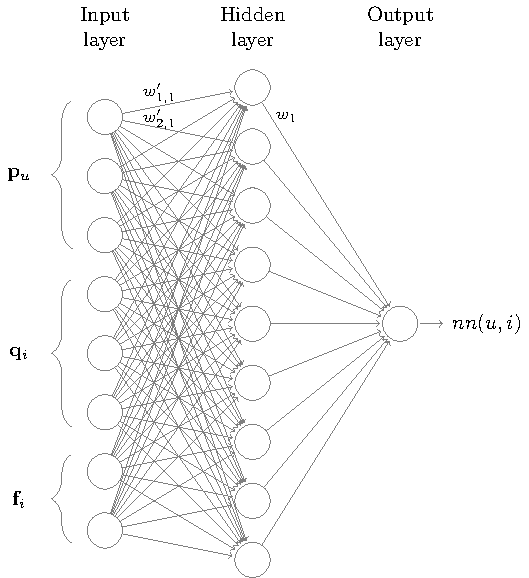
\includegraphics[width=0.7\linewidth]{./section-chapter1/figures/mfnn.pdf}
	\caption[MFNN: Neural Network]
	{MFNN: Neural Network}
	\label{f:mfnn}
\end{figure}

